Currently, we don't have Wi-Fi localization data for experienment. Instead, we decided to use offline dataset from *** and output the map data which can be regarded as the wifi data. To be noticed that the offline dataset should have closed loop otherwise it would be affected by the camera drift. Global bundle adjustment is engaged after the loop closure which means the drift is reduced or, in some extent, elminated. For simplication, we choose dataset 07 from *** and the map is shown at the Figure \ref{Track_original}.\\
First, since all the map data are stored in the keyframes which is consist of camera pose $R$ and translation $t$, we modified the original software and output the keyframes' data and timestamps. After that, we use Python script to process the data based on the math we discussed above and simulate the noise from the real Wi-Fi localization device. The processed map data is shown at the Figure \ref{Track_processed}. The script is attached in the appendix.
\begin{figure}
    \centering
    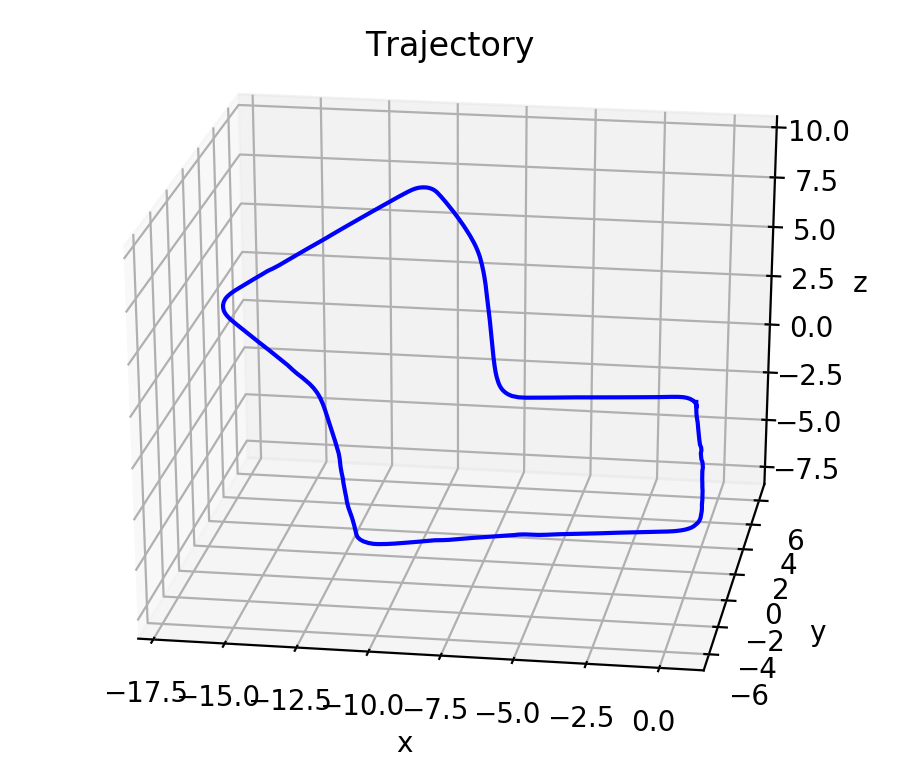
\includegraphics[scale=0.72]{Trajectory.png}
    \caption{Trajectory from Dataset}
    \label{Track_original}
\end{figure}
\begin{figure}
    \centering
    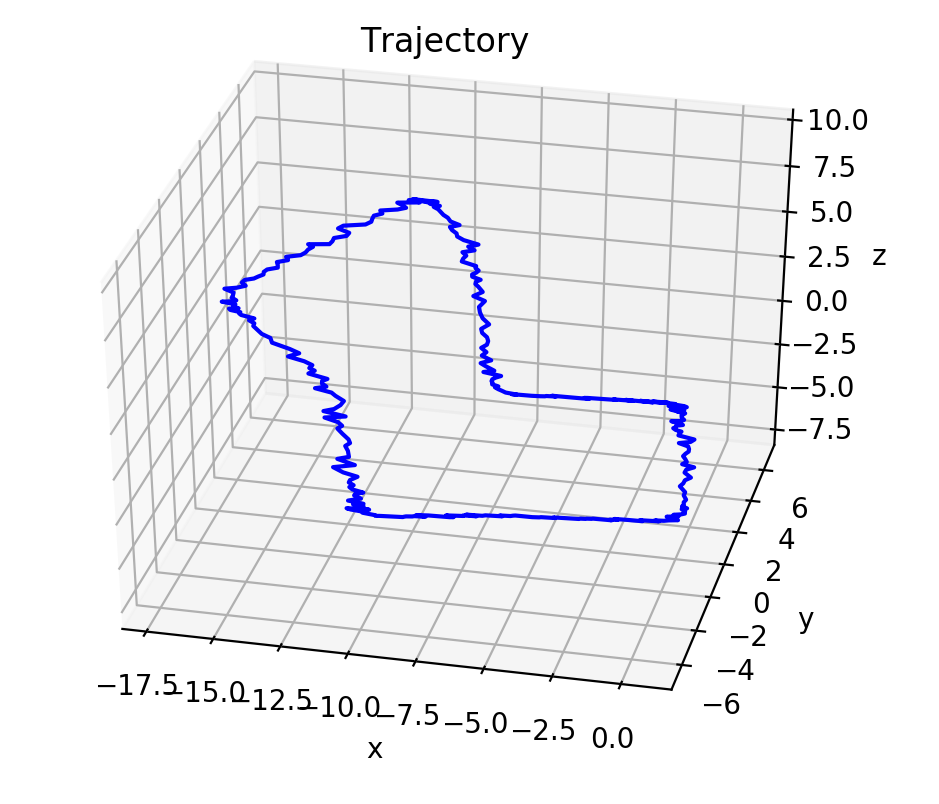
\includegraphics[scale=0.69]{Trajectory_1.png}
    \caption{Trajectory after Processed}
    \label{Track_processed}
\end{figure}